\documentclass[conference]{IEEEtran}

\ifCLASSINFOpdf
\else
\usepackage[dvips]{graphicx}
\fi

\usepackage{epsfig}
\usepackage{graphics}
\usepackage{graphicx}

\usepackage[cmex10]{amsmath}

\usepackage{flushend}


%\hyphenation{op-tical net-works semi-conduc-tor}


\begin{document}

\title{Mechanistic modeling of collective vehicular dynamics reproduces empirical features of congested traffic}

\author{\IEEEauthorblockN{R. Alfred Ajay Aureate and Sitabhra Sinha}
\IEEEauthorblockA{The Institute of Mathematical Sciences,\\
CIT Campus, Taramani, Chennai 600113, India\\
Email: alfredajay@imsc.res.in, sitabhra@imsc.res.in}}

\maketitle

%=============================================================================%

\begin{abstract}
Vehicular traffic is studied mostly as a network or a dynamical problem. Dynamical understanding of traffic provides a lot of insight about the microscopic aspects of traffic, that might be quite useful for improving traffic infrastructure with least effort. There has been a range of various complicated fluid dynamical models to extremely simple cellular automata (CA) models that have been proposed for decades. We've unified the positve aspects of those models and have come up with a simlple mechanistic model that could simulate various properties of traffic. We've described and shown how using this model one could reproduce the fundamental diagram (relation between mobility, flow and density of vehicles), time evolution of velocity and acceleration and the power-law behaviour of the congestion times as observed from empirical data in Indian cities. We've shown that the the heterogeneity of the vehicles is a very crucial factor in affecting the power-law behaviour of congestion times.

\end{abstract}

\IEEEpeerreviewmaketitle

%=============================================================================%

\section{Introduction}

%%%%%%%%%%%%%
As a result of the advancement in computing architecture and numerical techniques, large-scale social dynamics are nowadays modelled in a simpler manner using just the interactions between autonomous agents. Through such approach, the macroscopic changes can be observed at the level of the entire system by describing just the micro-dynamics of the individual constituents~\cite{Ball2003}. For example, the transition of the traffic state from free flowing to jammed state and vice versa \cite{Helbing2001}, \cite{Chakrabarti2007}.

Although vehicle traffic has been studied for decades using fluid dynamical models, after Nagel and Schreckenberg introduced a much simpler cellular automata model of highway traffic flow \cite{Nagel1992}, there has been an increased interest towards describing complicated patterns of traffic using elegant microscopic models. Yet, there has been very little work done regarding urban traffic.

Studying urban traffic turns out to have more significance both in terms of academical and economical point of view, as the study of traffic jams and their lifetimes might be helpful in building more efficient transport infrastructure in a city. Also, as mentioned earlier in \cite{Majith2015}, the congestion times (or the waiting times of vehicles in the jam) follows a power-law (as opposed to an exponential which would generally be expected for a memoryless random process), thereby making the study of congestion even more interesting.

By studying the critical factors that affects traffic congestion times, one would be able to deduce what aspects of traffic could be used to control and perhaps to overall reduce congestion time in traffic. Earlier \cite{Majith2016}, a kinetic Monte-Carlo model was introduced that explains how power-law characteristic of the waiting time emerges when there is some heterogeneity in the way cars respond to headway distances. Here, we've used acceleration-based updating scheme to represent reality more closely and to explain which specific aspect of heterogeneity plays a crucial role in characterizing the exponents of the power-law behavior of the waiting times.

\begin{figure}
%    \centering
{    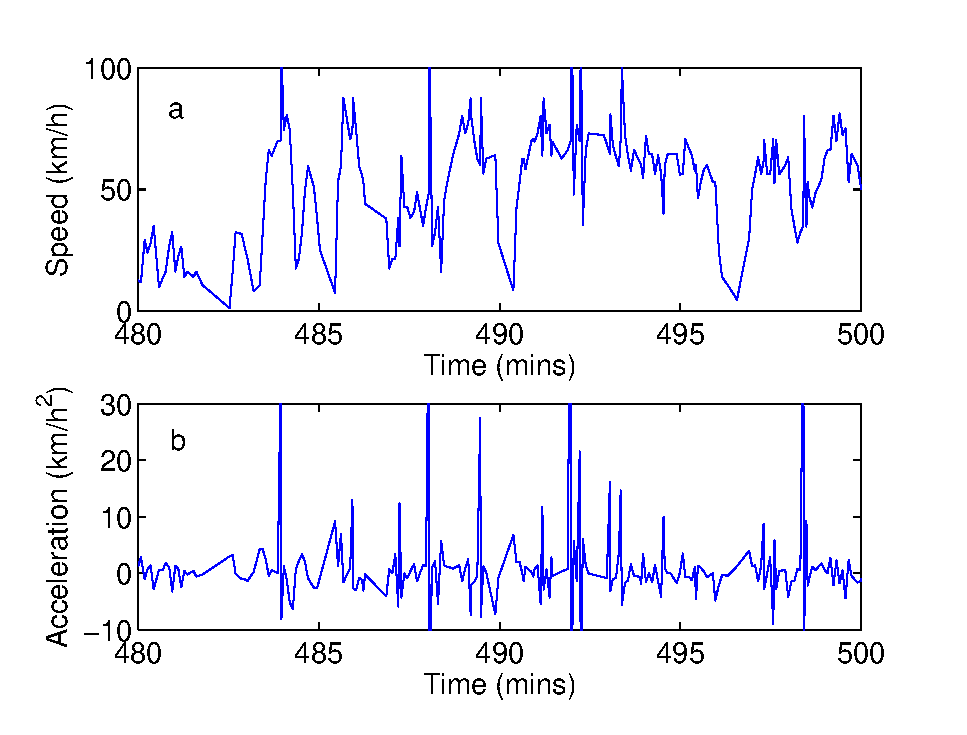
\includegraphics[width=9.0cm, angle=0]{fig1.eps}}
    \caption{Time evolution of (a) speed and (b) acceleration of an individual vehicle in New Delhi for the period 1:30pm - 1:50pm (IST) on Jan 10, 2013. }
    \label{taxi_acc}
\end{figure}

From the dataset obtained from \cite{traffline} (fig. \ref{taxi_acc}), we observe for a particular taxi in New Delhi (on 10th Jan, 2013) that the velocity varies rather in a relatively continuous fashion, whereas, the acceleration varies quite abruptly over time. This aspect is not captured by any of the earlier models.


%=============================================================================%

\section{Model}
%Bass model
The kinetic Monte Carlo model that had been introduced earlier in \cite{Majith2016} was majorly to explain the power-law characteristics of the waiting times observed in \cite{Majith2015} and the fundamental relation between mobility, flow and density (which is a general relation). But, in that model, the velocities are abruptly changed every time step (depending on the headway distance) which is not that case in real life as the empirical data suggests in \ref{taxi_acc}. Instead, the control mechanisms are in fact acceleration based, namely - accelerator or brake. So, in this paper we intend to improvise the velocity-based model to incorporate the acceleration-based controls and effects. Moreover, the earlier model was phenomenological, whereas this one is mechanistic. % This would in turn smoothen out the velocity vs time plot as expected from the empirical data.

Similar to the model in \cite{Majith2016}, here too we assume a single lane with fixed number of vehicles moving only in one direction. %In order to avoid boundary issues, a circular road is considered.
To avoid problems with maintaining constant the traffic density by adjusting the input and output rates, circular road is considered. Also, those vehicles are externally controlled by a signal which is placed at one end of the road. %This signal basically represents the cross-over traffic.
The signal controls cross traffic at an intersection (signal controlled characterizes urban traffic). Now, instead of just updating the velocities of each vehicle at every instant, we update acceleration as follows:

\begin{equation}
\begin{split}
    \frac{dx_{i}}{dt} &= v_{i}\\
    \frac{dv_{i}}{dt} &= -(\gamma_{i} + \xi(x,t))v_{i} + \beta_{i}\bigg(\frac{d_{i}-v^{rel}_{i}\tau_{i}}{d_{i}+1}\bigg)
\end{split}
\label{dxdv}\end{equation}

where,

% not sure if we can use $\gamma(1+\epsilon\xi(x.t))$

$\gamma_{i}$ : drag rate due to friction of the road surface for car $i$.

$\xi$ : space and time dependent perturbation ( $>0$ ) in the drag rate that affects just a random car for each time step, representing possibly a pothole or applying of brake, etc.

$\beta_{i}$ : maximum acceleration possible (by pressing %or applying
the accelerator).

$\tau_{i}$ : reaction time of the car-driver interface of car $i$.

$d_{i}$ : headway distance available in front of car $i$ to move without colliding. $d_{i}=|x_{i+1}-x_{i}|$, where $x_{i+1}$ and $x_{i}$ are positions of cars $i+1$ and $i$.

$v^{rel}_{i}$ : relative velocity of the car in front with respect to the car under consideration ($i$). $v^{rel}_{i}=v_{i+1}-v_{i}$.

Maximum velocity could then be given by, $v^{max}_{i}=\beta_{i}/\gamma_{i}$ (for a single car in an otherwise empty road $\frac{dv_{i}}{dt}=-\gamma_{i} v_{i} + \beta_{i}$)

In most of the figures, we either choose identical values of $\gamma$, $\beta$ and $\tau$ or random values for each car at the start of each simulation.%values remain the same though throughout the simulation
Without loss of generality, we pick those three parameter values for each car from a gamma distribution, so that we could analyze from a range of distributions. By averaging over several such realizations the probability distribution of the waiting time is calculated. This would therefore provide an insight as to which (inherent) characteristic of the car-driver-road system is crucial for the power-law behaviour of the waiting time. It has already been shown that the power-law could emerge just from simple dynamics, without even considering any network structure nor multi-lanes, in \cite{Majith2016}. The influence of external characteristics like the signal cycle, traffic density and duty ratio (of the signals), over the power-law behaviour will be published elsewhere \cite{PRL}.

The first term in the acceleration eqn. (\ref{dxdv}) represents the friction due to the road surface and it is proportional to the instantaneous velocity. Similarly, the second term represents the acceleration given by the driver for every time step. It is directly proportional to the headway distance available for the vehicle in front. We've used an hyperbolic function just to ensure that there is a saturation to maximum value of acceleration. Since there would be a lag in terms of the car-driver system to respond, the actual headway distance ($d-v^{rel}\tau$) would be lower than the physical headway distance, $d$. Since $d\gg v_{rel}\tau$ usually,
\[\frac{d_{i}-v^{rel}_{i}\tau_{i}}{d_{i}-v^{rel}_{i}\tau_{i}+1}\approx \frac{d_{i}-v^{rel}_{i}\tau_{i}}{d_{i}+1}\]

Based on those equations (\ref{dxdv}) for all cars, the time step $dt$ for progressing time is calculated based on two conditions: i) None of the cars collide with the cars in front while the vehicles progress with constant acceleration during $dt$. ii) None of the cars' velocity goes below zero. The largest such $dt$ value is chosen for updating. At time $n$ (using Newton's 2nd law we arrive at),

\begin{equation}
    dt_{n} = \min_{i}\left( \frac{-v_{i,n-1} + \sqrt{v_{i,n-1}^2 + 2a_{i,n-1}d_{i,n-1}}}{a_{i,n-1}}\right)
\end{equation}

where $v_{i,n-1}$ is velocity, $a_{i,n-1}$ is acceleration and $d_{i,n-1}$ is headway distance at time $n$ for the car $i$. $dt_{n}$ is now the time step at time $n$. This adaptive step-size allows us to mimic continuous-time, continuous-space dynamics more accurately. Note that the determinant (or the expression inside the square root) always remains non-negative as it is just the square of the final velocity (or the velocity just after the time step).

%=============================================================================%
\section{Results}
 %-----------------------------------------------------------------------------%

We have considered the vehicular density (i.e., the fraction of road surface occupied by cars) to be $0.5$ in all cases reported here. Also, the signal cycle is about 60 time units for each red and green light. Given that, we observe from Fig. \ref{acc_t}(a) that when the cars and drivers are identical, the acceleration is a periodic function that synchronizes with the signal cycle. On the other hand, in fig. \ref{acc_t}(b) where the agents (car-driver systems) are assumed to be non-identical, the acceleration doesn't behave periodically, but rather in an erratic fashion. In fact, the maximum magnitude in both positive and negative directions has increased, which could possibly mean that the agents are applying stronger braking/acceleration because of the unpredictability. %quite behaving in an unpredictable and "aggressive" manner.

\begin{figure}
%    \centering
{    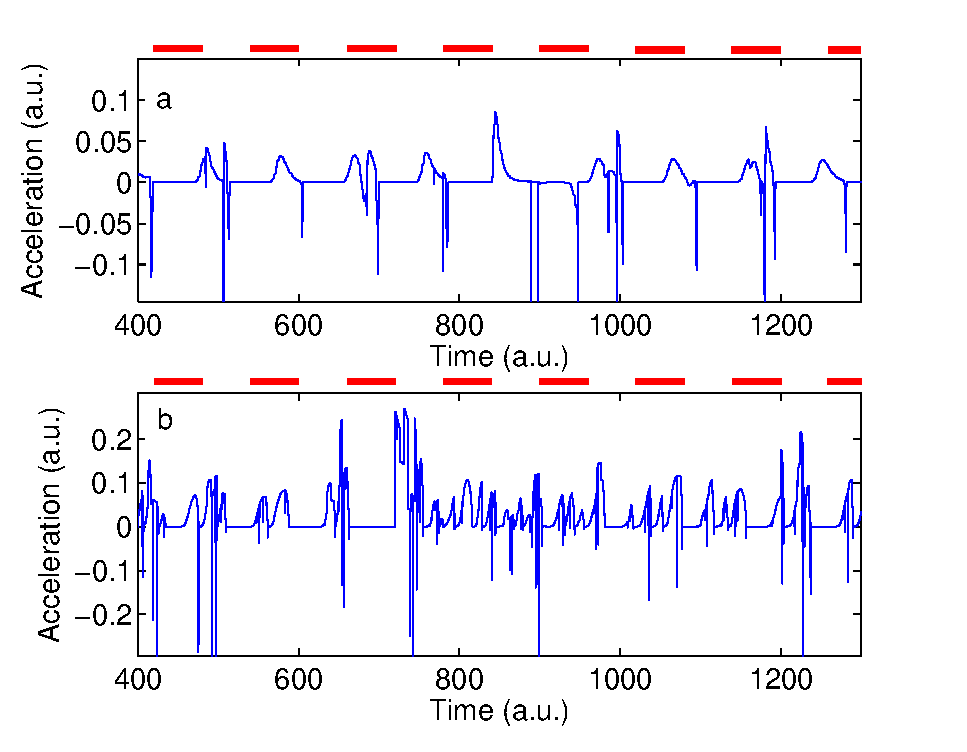
\includegraphics[width=9.0cm, angle=0]{fig2_v2.eps}}
    \caption{Time evolution of acceleration for an individual simulated vehicle in the model described in the text for (a) the homogeneous case when all vehicles are identical and (b) the heterogeneous case where the vehicles have distinct (randomly chosen) characteristics. For (a) all the cars have $\gamma=0.2$, $\beta=0.2$ and $\tau=0.3$. For (b), the average values over all 100 cars of these parameters are $\langle \gamma \rangle =0.02$, $\langle \beta \rangle =0.2$ and $\langle \tau \rangle =0.03$. In both cases, the noise $\xi$ is chosen from the uniform distribution $[0.0.6]$. The periods during which the signal is red is indicated with color red horizontal bars shown along the top of the figure.}

%    \caption{Variation of acceleration over time from the simulation. The traffic signal is marked with red. a) shows the variation of the instantaneous acceleration for a single car when we assume all identical cars with identical parameter values. b) similarly shows the variation of instantaneous acceleration when the parameter values for each car is different from each other.}
    \label{acc_t}
\end{figure}


Such contrasting pattern in the acceleration gets smoothened out in the velocity variation as time progresses, fig \ref{vel_t}. Even though the velocity variation in fig. \ref{vel_t}(b) is more smooth than the one with the stochastic noise in \cite{Majith2016}, it still has spikes and appears to be more unpredictable compared to fig. \ref{vel_t}(a). Again, because of higher maximum magnitudes for acceleration, we observe higher maximum values of speed also in fig. \ref{vel_t}(b), even though overall average velocity of the system remains almost the same in both cases.


\begin{figure}
%    \centering
{    \includegraphics[width=9.0cm, angle=0]{fig3_v3.eps}}
    \caption{Time evolution of velocity for an individual simulated vehicle in the model described in the text for (a) the homogeneous case when all vehicles are identical and (b) the heterogeneous case where the vehicles have distinct (randomly chosen) characteristics. For (a) all the cars have $\gamma=0.2$, $\beta=0.2$ and $\tau=0.3$. For (b), the average values over all 100 cars of these parameters are $\langle \gamma \rangle =0.02$, $\langle \beta \rangle =0.2$ and $\langle \tau \rangle =0.03$. In both cases, the noise $\xi$ is chosen from the uniform distribution $[0.0.6]$. The periods during which the signal is red is indicated with color red horizontal bars shown along the top of the figure. (c) The complementary cumulative probability distribution of speed of vehicles when they are a specific headway distance from the preceding vehicle (shown for four different values) exhibits an exponential behaviour. (d) The mean velocity as a function of the headway distance $d$ shows a sigmoidal nature. The broken curve is a theoretical fit to the simulated data shown using circles.}

%    \caption{Variation of velocity over time in the simulation. Blue line shows the instantaneous velocity of a single car, whereas the dotted green line represents the instantaneous average velocity across the system. The swapping of the traffic signal is marked by red where marking over '1' represents the red signal and '0' represents green signal. a)  shows velocity variation over time when the cars are assumed to be 'identical' to each other, in the sense that the car-specific parameters are all same for each one of them. b) shows the velocity variation when the cars are assigned with different parameter values, namely $\gamma$, $\beta$ and $\tau$.}
    \label{vel_t}
\end{figure}

By comparing the figures \ref{acc_t}(b) and \ref{vel_t}(b) with figures \ref{taxi_acc}(b) and \ref{taxi_acc}(a) respectively, we could quite conclude that our model's prediction about the evolution of velocity or acceleration over time agrees well with the empirical data.

Also, from the figure \ref{vel_t}(c) and (d), we notice that the exponential fluctuation for velocity and the sigmoidal relation between headway distance and velocity assumed in \cite{Majith2016} is satisfied by this model too, thereby making this model a more general one.

In fig. \ref{spacetime}, we plot the space-time trajectory of each car as it moves along the single-lane road towards the signal (marked on the right end). We notice from the plot on the top of fig. \ref{spacetime} that the cars start behaving in a periodic and deterministic fashion when the agents are assumed to be identical, whereas there arises a lot of random perturbations in the trajectory of the cars when the agents are assumed to be non-identical to each other (bottom of fig. \ref{spacetime}). So, when the agents are non-identical, lot of internal perturbations start arising, even if there is no effect of a signal. In the simulation, it has been made sure that the cars never collide at any instant, so, we see that the trajectories never intersect nor touch each other. %Such constraint is ensured by picking the time step in such a way that the cars move with constant acceleration over the duration of that time step without colliding nor decreasing it's velocity below zero, meaning we assume that cars rather stop instead of moving in the reverse direction.


\begin{figure}
%    \centering
{    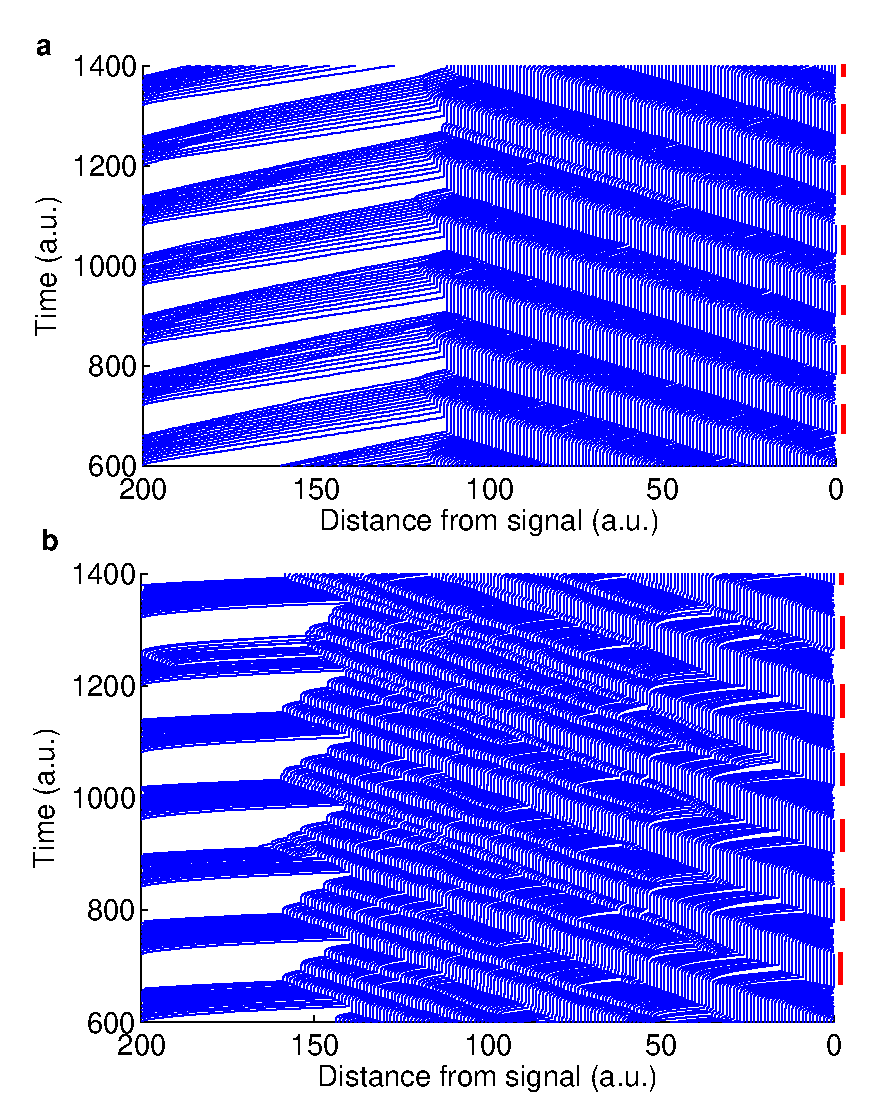
\includegraphics[width=9.0cm, angle=0]{fig4.eps}}
    \caption{Space-time trajectories of vehicles...}

%    \caption{Both the plots show the space-time evolution of all cars. Each line represents the space-time trajectory of a single car. Traffic signals are marked with red on the right side for reference. When we consider identical car-driver system (top), the space-time evolution of the cars kind of synchronize with each other and resembles very close to that of the deterministic case in \cite{Majith2016}, whereas we could observe (bottom) that there are various other perturbations causing an increase in the length of the jam when the car-driver systems are considered to be non-identical. Interestingly, unlike in the identical case (top), the non-identical nature of individuals (bottom) results in the reduction of the effect of any perturbation as it propagates backwards.}
    \label{spacetime}
\end{figure}



The fundamental diagram in fig. \ref{fund} shows how mobility $\langle v \rangle$ and flow $J$ varies as a function of density $\rho$.

Density here is defined as the number of cars per unit car length of the road, $\rho=\frac{P}{L}$, where $P$ is the number of cars and $L$ is the road length.

Mobility is given by,
\[\langle v \rangle = \frac{\text{Total distance travelled by all cars during simulation}}{(\text{Total duration of simulation})P}\]
and flow is $J=\langle v \rangle \rho$. The dotted red line shows how the transition from free flow to jammed state occurs in an highway (meaning in the absence of signals). From the blue line plot, we observe that, unlike in an highway, the transition is not abrupt, but rather the flow in the traffic flow with intersections (meaning with traffic signals) is actually similar for a wide range of density values, causing a flattened plateau, fig. \ref{fund}(b). The mobility becomes more concave as a function of density, fig. \ref{fund}(a).


\begin{figure}
%    \centering
{    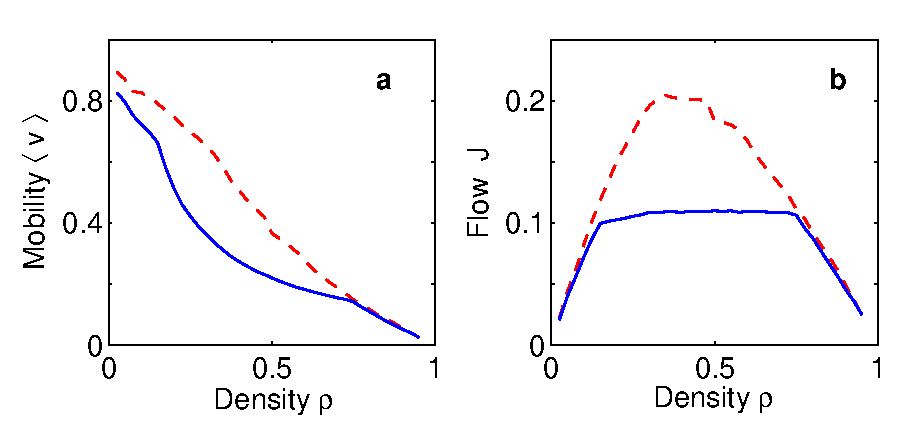
\includegraphics[width=9.0cm, angle=0]{fig5.eps}}
    \caption{a) Mobility vs density. b) Flow vs density. Blue line is for the case when there is signal and red dotted line is when there is no signal, meaning if it was just an highway}
    \label{fund}
\end{figure}

We find that using our acceleration-based model, the congestion times follow a power-law distribution, 
\begin{equation}
    p(T=\tau) \sim \tau^{-\alpha}
\end{equation}

with varying exponent values $\alpha$ (where $\alpha$ is a non-negative real number), as shown in fig. \ref{power_law_abt} and fig. \ref{power_law_gam}. When the agents are assumed to be identical, we've noticed from previous figures that the system very closely resembles a deterministic one. So, we would only be considering the non-identical case here. As the values of $\xi$, $\langle \gamma \rangle$, $\langle \beta\rangle$ and $\langle\tau \rangle$ are varied, the power-law distribution of the congestion times have exponents very close to $1.7-2.2$. But, when we assume stochastic fluctuations in the parameter values, meaning heterogeneity of the parameters $\gamma$, $\beta$ and $\tau$, we then get a range of power-law exponents, from $1.8-3.2$ for different choice of shape parameter of the gamma distribution (especially for sub-exponential distributions), as shown in fig. \ref{power_law_gam}.



\begin{figure}
%    \centering
{    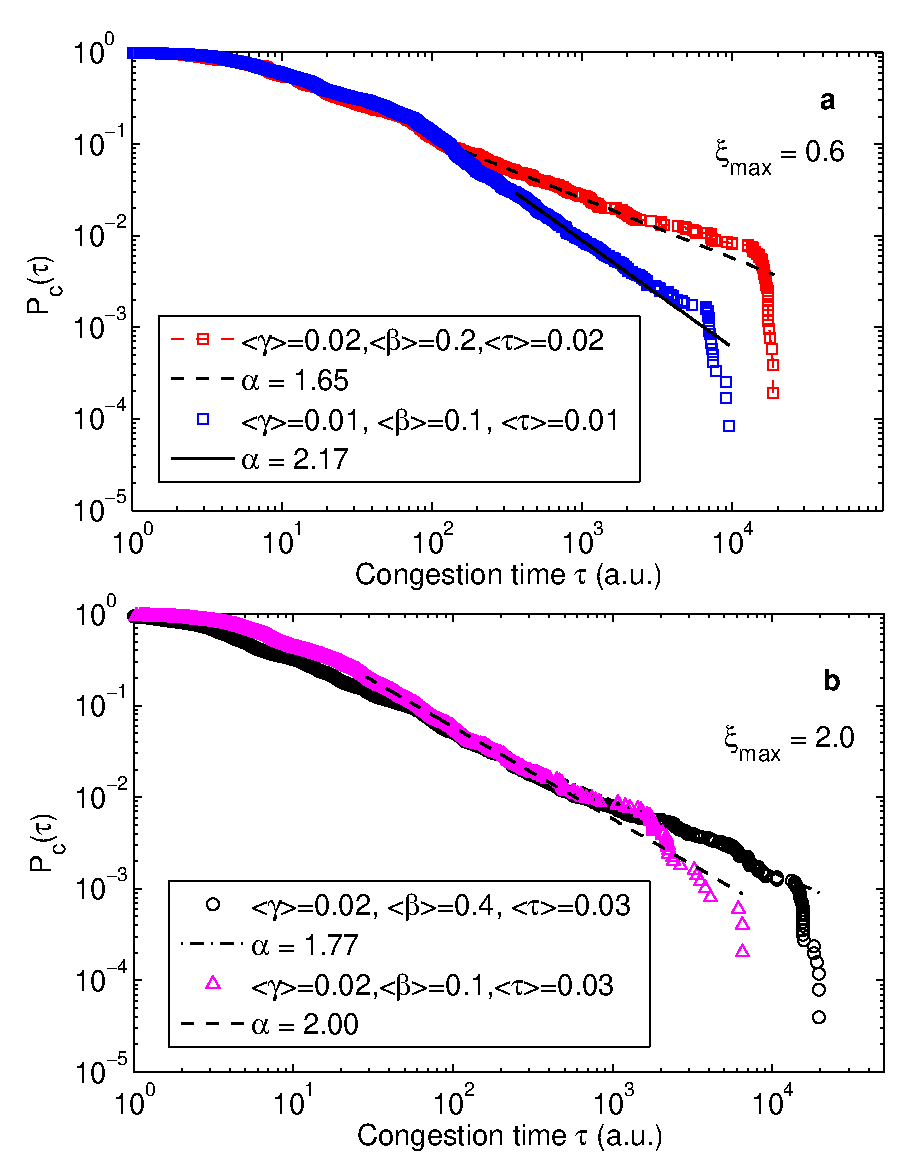
\includegraphics[width=9.0cm, angle=0]{fig6.eps}}
    \caption{Complementary cumulative distribution of the congestion time when we consider different mean values for different acceleration parameters.}
    \label{power_law_abt}
\end{figure}

\begin{figure}
%    \centering
{    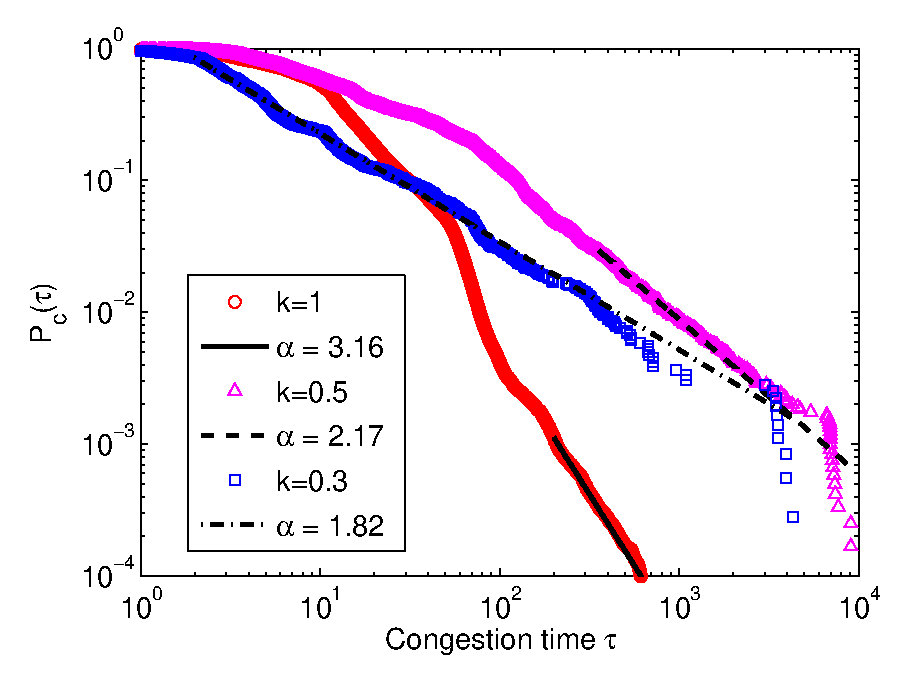
\includegraphics[width=9.0cm, angle=0]{fig7.eps}}
    \caption{Complementary cumulative distribution of the congestion time for different type of heterogeneity for the acceleration parameters. Basically, the shape parameter of the gamma distribution is varied to represent a wide range of distributions.}
    \label{power_law_gam}
\end{figure}

The exponent values of the power-law is obtained using the Maximum-Likelihood method given by Clauset., et. al. in \cite{Clauset2009}. This provides a best power-law fit to the distribution that is obtained from the simulation.


\section{Conclusion}
In this report, we've presented a novel approach towards modelling the traffic congestion using a microscopic Monte-Carlo model. Following Newton's laws, with some fluctuations in terms of the non-identical nature of the car-driver system, we have shown that one could obtain waiting times following a power-law distribution. This therefore does not introduce any fluctuation directly into the dynamics, as as done in \cite{Majith2016}. Moreover, the range of exponent values, $\alpha$'s, agrees very well with the range of exponent values obtained from empirical data of various Indian urban cities, namely Bangalore, Bombay and Delhi \cite{Majith2016},\cite{Majith2015}.

%=============================================================================%

\section*{Acknowledgments}

The authors would like to thank Krishna Jagannathan for help in accessing the GPS trace data analyzed here, Abdul for initiating the analyses of traffic using microscopic Monte-Carlo models, Soumya Easwaran, Shakti Menon and K Chandrashekar for assistance in data analysis, and IMSc for providing access to the high-performance computing facility.
This research was supported in part by the ITRA Media Lab Asia 
project ``De-congesting India's Transportation Network'' and IMSc Complex Systems Project.

%=============================================================================%
%=============================================================================%

\begin{thebibliography}{1}
\bibitem{Ball2003}
{P.~Ball, ``The physical modelling of human social systems,'' {\em
Complexus}, vol. 1, pp.~190–206, 2003.}

\bibitem{Helbing2001}
{D.~Helbing, ``Traffic and related self-driven many-particle
systems,'' {\em Rev. Mod. Phys.}, vol. 73, pp.~1067-1141, 2001.}

\bibitem{Chakrabarti2007}
{B.~K.~Chakrabarti, A.~Chakraborti and A.~Chatterjee, Eds. {\em
Econophysics and Sociophysics: Trends and perspectives}. 
Weinheim: Wiley-VCH, 2007.}

\bibitem{Nagel1992}
{K.~Nagel and M.~Schreckenberg, ``A cellular automaton model
for freeway traffic,'' {\em J. Phys. I}, vol. 2, pp.~2221–2230, 1992.}

\bibitem{Majith2015}
{N.~Abdul Majith and S.~Sinha, ``Statistics of stop-and-go traffic: Emergent properties of congestion 
behavior arising from collective vehicular dynamics in an urban environment,'' in {\em Proceedings of the 
7th International Conference on Communication Systems and Networks (COMSNETS)}, Bangalore, 2015, pp.~1-4.}

\bibitem{Majith2016}
{Majith NA and Sinha S (2016) Dynamics of urban traffic congestion: A kinetic Monte Carlo
approach to simulating collective vehicular dynamics. Paper presented at the 8 th International
Conference on Communication Systems and Networks (COMSNETS), The Chancery Pavillion, Bangalore, 2016}

\bibitem{traffline}
http://www.traffline.com/

\bibitem{Clauset2009}
{A.~Clauset, C.~R.~Shalizi and M.~E.~J.~Newman, ``Power-law distributions 
in empirical data,'' {\em SIAM Review}, vol. 51, pp.~661-703, 2009.}

\bibitem{PRL}
{"Dynamics of traffic congestion" (to be published elsewhere)}

%\bibitem{Wheeler1989}
%{J.~A.~Wheeler, ``Information, physics, quantum: The search for
%links,'' in {\em Proceedings of the 3rd International Symposium on the
%Foundations of Quantum Mechanics}, Tokyo, 1989, pp.~354-368.}

%\bibitem{Zurek1990}
%{W.~H.~Zurek, Ed., {\em Complexity, Entropy, and Physics of
%Information}. New York: Addison-Wesley, 1990.}

%\bibitem{Sinha2006}
%{S.~Sinha, ``Phase transitions in the computational complexity of elementary
%cellular automata,'' in {\em Unifying Themes in Complex Systems},
%A.~A.~Minai and Y.~Bar-Yam, Eds. Berlin: Springer, 2006, 
%pp.~337-348.}

\end{thebibliography}

%=============================================================================%
%=============================================================================%

% that's all folks
\end{document}
